\documentclass{article}


\usepackage[english]{babel}
\usepackage{listings}
\usepackage[letterpaper,top=2cm,bottom=2cm,left=3cm,right=3cm,marginparwidth=1.75cm]{geometry}

\usepackage{amsmath}
\usepackage{graphicx}
\usepackage{listings}

\lstset{language=Python}
\title{COSC 343: Test 2}
\author{Micah Sherry}

\begin{document}
\maketitle
\section{Fresnel Integrals}
	The intesity of difracted light near a straight edge is determied by the values of the Fresnel Integrals: 
	$$C(x) = \int_{0}^x cos(x)dx $$ and $$S(x) = \int_{0}^x sin(x)dx $$
	Use a quadrature routine to evaluate the integrals for enough values of x to draw a smooth plot of C(x) and S(x) over the range
	$0 \le x \le 5$

	For my quadrature routine I used a composite four point Guassian routine. 
	For the Fresnel integrals I set the number of subintervals to $2(|x|+1)$.     
	To get a smooth plot on the interval [0,5] I needed to use 140 x points .
\subsection*{Code:}
	\lstinputlisting[]{../Fresnel.py}
\subsection*{Plots:}
	\begin{figure}[hbt!]
		\centering
		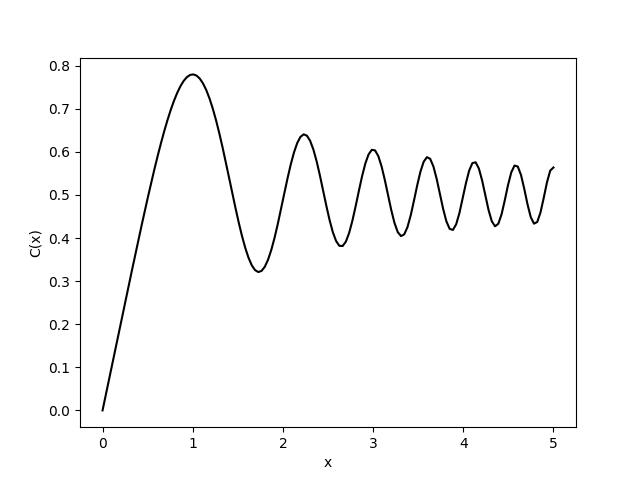
\includegraphics[width=.75\linewidth]{C(x)_plot.png}
		\caption{Fresnel integral C(x)}
		\label{fig: Fresnel integrals C(x)}
	\end{figure}
	
	\begin{figure}[hbt!]
		\centering
		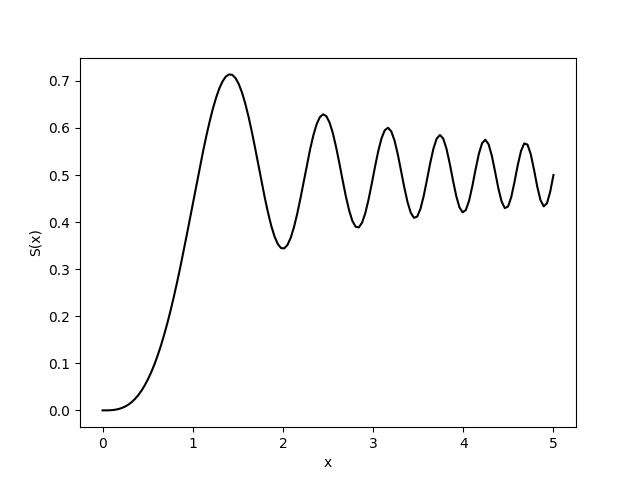
\includegraphics[width=.75\linewidth]{S(x)_plot.png}
		\caption{Fresnel integral S(x)}
		\label{fig: Fresnel integrals S(x)}
	\end{figure}
\end{document}

